\chapter[Diskussion des aktuellen Stands der Forschung und Praxis]{Diskussion des aktuellen Stands der Forschung und Praxis\footnote{Sprachlich geglättet durch ChatGPT-5}}
\label{chapter:Stand_Forschung_und_Praxis}

\section{Digitale Modelle in der Fertigungsindustrie}

Die Entwicklung digitaler Modelle von Maschinen und Anlagen ist ein zentrales Element der Industrie 4.0. Durch die bessere Vernetzung von Systemen sowie Fortschritte in der Datenanalyse, insbesondere durch KI, steigt auch die Forschung und Nutzung an digitaler Abbildungen.\footnote{Vgl. \cite[S. 108952]{fuller_digital_2020}} Im Folgenden soll näher auf den Stand der Forschung in diesem Bereich sowie Entwicklungstrends und aktuelle Herausforderungen eingegangen werden.

\subsection{Begriffsabgrenzung: Digitales Modell, Digitaler Schatten, Digitaler Zwilling}
Obwohl in der Literatur häufig pauschal von Digitalen Zwillingen die Rede ist, lässt sich eine Unterscheidung in Digitales Modell, Digitaler Schatten und Digitaler Zwilling vornehmen. Diese Begriffe werden fälschlicherweise oftmals synonym verwendet, obwohl sie einige signifikante Unterscheidungen in ihrer Systemarchitektur aufweisen.\footnote{Vgl. \cite[S. 1017]{kritzinger_digital_2018}} Zwar existieren keine einheitlichen Definitionen,\footnote{Vgl. \cite[S. 350]{liu_review_2021}; \cite[S. 108953]{fuller_digital_2020}} jedoch unterscheidet eine gängige Klassifizierung die drei Formen der digitalen Abbildungen basierend auf dem Grad der Datenintegration zwischen dem physischen und dem digitalen System.\footnote{Vgl. \cite[S. 108953]{fuller_digital_2020}; \cite[S. 1017 f.]{kritzinger_digital_2018}}

\textbf{Digitales Modell}

Bei einem digitalen Modell handelt es sich um eine digitale Repräsentation eines existierenden oder geplanten Objekts. Es findet kein automatisierter Austausch von Daten statt, der Datenfluss erfolgt also in beide Richtungen, vom physischen zum digitalen Objekt und umgekehrt, ausschließlich manuell. Das Modell kann durchaus auf Basis realer Daten erstellt werden oder diese nutzen, jedoch passiert dieser Austausch nicht automatisch, wodurch die beiden Systeme keinerlei Einfluss aufeinander haben.\footnote{Vgl. \cite[S. 108953]{fuller_digital_2020}}

\textbf{Digitaler Schatten}

Von einem digitalen Schatten ist häufig die Rede, wenn der Datenfluss einseitig automatisiert ist. Daten vom physischen Objekt fließen automatisch in die digitale Repräsentation ein, während umgekehrt der Fluss vom digitalen in das physische Objekt weiterhin ausschließlich manuell stattfindet. Dies führt dazu, dass eine Veränderung des physischen Objekts einen direkten Einfluss auf das digitale Objekt hat, allerdings nicht umgekehrt.\footnote{Vgl. \cite[S. 1017]{kritzinger_digital_2018}}

\textbf{Digitaler Zwilling}

Der Digitale Zwilling ist die Architektur mit dem höchsten Grad der Datenintegration zwischen physischem und digitalem Objekt. Hierbei findet der Datenfluss in beide Richtungen automatisiert statt, beide Systeme sind also miteinander verbunden und haben beidseitig einen direkten Einfluss aufeinander. Alle Informationen, welche von dem realen System gesammelt werden können, sollen auch in die digitale Repräsentation einfließen, wodurch diese das physische System spiegeln soll. Änderungen des physischen Objekts führen also direkt zu Änderungen des digitalen Objekts und umgekehrt.\footnote{Vgl. \cite[S. 1017]{kritzinger_digital_2018}; \cite[S. 108963]{fuller_digital_2020}}

Oftmals wird fälschlicherweise pauschal von einem Digitalen Zwilling gesprochen, wobei es sich in vielen Fällen nicht um einen tatsächlichen Digitalen Zwilling mit einem bidirektionalen Fluss an Daten handelt.\footnote{Vgl. \cite[S. 1020]{kritzinger_digital_2018}}

\subsection{Forschungsstand und Entwicklungstrends}
Frühere Arbeiten konzentrierten sich überwiegend auf die Forschung und die Entwicklung von Konzepten und weniger auf konkrete Einsatzmöglichkeiten in der Fertigung.\footnote{Vgl. \cite[S. 1018 ff.]{kritzinger_digital_2018}} Jedoch lässt sich hier ein klarer Wandel erkennen, welcher immer mehr Forschung zum empirischen Einsatz von Digitalen Zwillingen, Modellen und Schatten aufzeigt, während auch die Forschung in der Fertigungsindustrie zunimmt.\footnote{Vgl. \cite[S. 349]{liu_review_2021}}

\subsection{Rolle der \acs{KI} und einhergehende Herausforderungen}
\ac{KI}-Anwendungen in Verbindung mit digitalen Zwillingen wurden zunächst selten erforscht und eingesetzt\footnote{Vgl. \cite[S. 352 ff.]{liu_review_2021}}, jedoch wird dieser Trend zunehmend populärer.\footnote{Vgl. \cite[S. 1]{mikolajewska_generative_2025}} \ac{KI} stand anfangs noch weniger umfangreich am Rande des Einsatzes,\footnote{Vgl. \cite[S. 352 ff.]{liu_review_2021}}gewinnt jedoch mittlerweile in unterschiedlichen Einsatzfeldern, insbesondere bei der Fehlererkennung und -klassifizierung sowie vorausschauender Wartung (engl. \textit{Predictive Maintenance}), immer mehr von Bedeutung. Damit werden auch Probleme, welche sich beim Training von \ac{KI}-Modellen, wie z.B. zu wenige oder einseitige Daten, immer relevanter.\footnote{Vgl. \cite[S. 1]{mikolajewska_generative_2025}} Insbesondere der Einsatz von Digitalen Modellen zur Generierung solcher Trainingsdaten ist ein hochaktuelles Forschungsthema, welches sich noch in einem frühen Stadium befindet und in der aktuellen Forschung bislang unterrepräsentiert ist. Hier besteht klar ein weiterer Forschungsbedarf.

\subsection{Nutzen und Anwendungsfelder in der Fertigung}
Der Einsatz digitaler Abbildungen in der Fertigung bietet vielfältige Vorteile. Durch diese Modelle ergeben sich Möglichkeiten wie die Echtzeit-Überwachung und der damit einhergehenden schnellen Reaktionsfähigkeit auf Anomalien, der Engpasskontrolle oder der Produktionsplanung und -steuerung.\footnote{Vgl. \cite[S. 352 ff.]{liu_review_2021}; \cite[S. 23]{alfaro-viquez_comprehensive_2025}} Außerdem ist es möglich, Simulation von Maschinen oder Anlagen vor ihrem tatsächlichen physischen Einsatz durchzuführen.\footnote{Vgl. \cite[S. 7]{alfaro-viquez_comprehensive_2025}} Sie ermöglichen des Weiteren die risikofreie Durchführung gefährlicher oder kostenintensiver Prozesse.\footnote{Vgl. \cite[S. 6]{zaripov_creation_2025}} Digitale Repräsentationen leisten somit einen wesentlichen Beitrag zur Erhöhung von Sicherheit, Qualität, Flexibilität und Effizienz in der industriellen Fertigung.


\section[Synthetische Bilddaten für das Training von KI-Modellen]{Synthetische Bilddaten für das Training von \ac{KI}-Modellen}
\label{sec:synthetische_daten_section}

Durch das Wachstum von \ac{DL} und \ac{CV} steigt auch der Bedarf an großen Mengen von annotierten und qualitativ hochwertigen Datensätzen.\footnote{Vgl. \cite[S. 767]{monnet_investigating_2024}} Die Beschaffung solcher Datensätze bringt jedoch insbesondere im industriellen Umfeld eine Vielzahl von Herausforderungen mit sich. Das Erstellen umfangreich und diverser Datensätze ist oftmals ressourcen- und zeitaufwendig sowie kostspielig und zudem menschlichem Fehler unterlegen.\footnote{Vgl. \cite[250]{urgo_monitoring_2024}} Primär im industriellen Umfeld fehlt es außerdem häufig an ausreichend Bildern mit tatsächlichen Fehlerfällen, da diese in der Realität vergleichsweise selten auftreten.\footnote{Vgl. \cite[S. 768]{monnet_investigating_2024}} Im Folgenden werden daher mögliche Lösungsansätze für diese Problematik durch die Nutzung synthetischer Daten vorgestellt und diskutiert.

\subsection{Potenziale synthetischer Daten}
Um die herausgestellten Probleme zu adressieren, rückt das Konzept der Generierung synthetischer Daten immer mehr in den Fokus der Forschung. Das Ziel ist es hierbei, durch unterschiedliche Ansätze schnell und kostengünstig möglichst realitätsnahe und umfangreiche Datensätze in praktisch unbegrenztem Umfang zu generieren, welche anschließend für das Training von \ac{KI} Modellen verwendet werden können. Auch eine präzise, pixelgenaue Annotation wird hierdurch ermöglicht.\footnote{Vgl. \cite[S. 768]{monnet_investigating_2024}; \cite[S. 250]{urgo_monitoring_2024}} Ein weiterer Vorteil ist die Möglichkeit, schon vor dem Start der Produktion Bilddaten generieren und Modelle für den konkreten Anwendungsfall trainieren zu können.\footnote{Vgl. \cite[S. 768]{monnet_investigating_2024}} 

\subsection{Herausforderungen beim Einsatz synthetischer Daten}
Es ergeben sich bei der Nutzung synthetischer Daten jedoch dennoch diverse Probleme, von denen insbesondere die Herausforderung des \textit{Domain Gaps}, im Mittelpunkt der Forschung steht. Bei dem \textit{Domain Gap} handelt es sich um das Problem, dass Modelle, welche auf synthetischen Daten trainiert wurden, Schwierigkeiten bei der Übertragbarkeit auf reale Anwendungsfälle aufzeigen.\footnote{Vgl. \cite[S. 768]{monnet_investigating_2024}} Ein Grund hierfür kann ein unzureichender Realismus der synthetischen Daten sein, welcher die Komplexität der realen Welt nicht ausreichend widerspiegelt, was durch die Arbeit von \cite{boikov_synthetic_2021} zu sehen ist. In ihrer Studie wurden Modelle auf die Erkennung von Stahlfehlern trainiert. Diese erzielten auf den synthetischen Daten gute Ergebnisse, die Genauigkeit nahm bei Tests auf realen Daten jedoch merklich ab.\footnote{Vgl. \cite[S. 8]{boikov_synthetic_2021}} Es ist dabei allerdings zu berücksichtigen, dass dieses Problem maßgeblich vom Anwendungsfall und der für diesen erforderlichen Detaillierungsgrad abhängt. In Fällen, wie beispielsweise der Erkennung von Objektrotationen, zeigen \cite{manettas_synthetic_2021}, dass auch mit weniger realistischen synthetischen Daten ein erfolgreiches Modell trainiert werden kann.\footnote{Vgl. \cite[S. 241 f.]{manettas_synthetic_2021}} 
%\textcolor{red}{Sollte hier auch auf Aspekte eingegangen werden, wie dass die besten Ergebnisse mit einer hybriden Methode, durch Training auf synthetischen und fine-tuning auf realen Daten, erzielt werden konnten?
Es kann also festgestellt werden, dass es in diesem Bereich weiterer Forschung bedarf.\footnote{Vgl. \cite[S. 772]{monnet_investigating_2024}}

Ein weiteres Problem bei der Nutzung synthetischer Daten stellt außerdem das sogenannte \textit{Over-Labelling} dar. Hierbei werden in den Trainingsbildern Merkmale als Fehler markiert, welche durch einen menschlichen Inspektor gar nicht erkannt werden könnten, beispielsweise aufgrund des Blickwinkels oder einer geringer Sichtbarkeit des Fehlers. Dies führt dazu, dass das Modell später auch unkritische Merkmale als Fehler klassifiziert und somit die Anzahl an \ac{FP} erhöht wird.\footnote{Vgl. \cite[S. 4431]{fulir_synthetic_2023}}

\subsection{Methoden zur Generierung synthetischer Daten}
Um solche synthetischen Daten zu generieren, haben sich verschiedene Ansätze entwickelt, welche sich in verschiedene Kategorien einteilen lassen, auf welche im Folgenden näher eingegangen wird:\footnote{Vgl. \cite[S. 4426 f.]{fulir_synthetic_2023}}

\textbf{Generative Modelle}

Zu einem populären Ansatz zur Erzeugung synthetischer Daten mit generativen Modellen gehören \acp{GAN}. \acp{GAN} bestehen aus einem Generator und einem Diskriminator, wobei der Generator synthetische Daten erzeugt und der Diskriminator versucht, zwischen echten und generierten Daten zu unterscheiden. Beide Netzwerke lernen dabei gegenseitig voneinander und werden gemeinsam optimiert, wodurch der Generator zunehmend realistischere Daten erzeugt.\footnote{Vgl. \cite[S. 1010]{jain_synthetic_2022}}
Allerdings ist das Problem hierbei, dass für das effektive Training von solchen \ac{GAN}-Modellen immer noch eine signifikante Menge an echten Trainingsdaten erforderlich ist.\footnote{Vgl. \cite[S. 768]{monnet_investigating_2024}} 
%\textcolor{red}{Es könnten noch Alternativen zu \acp{GAN}, wie VAEs, RBMs oder Helmholtz Machines genannt werden oder auch Diffusionsmodelle}

\textbf{Computergrafik (Rendering-basierte Methode)}

Bei rendering-basierten Methoden wird eine Simulationsumgebung entwickelt, welche die realen Abläufe und Zustände widerspiegelt. 
Der Vorteil ist hierbei, dass einfach verschiedene Parameter, wie beispielsweise Lichtverhältnisse oder Kamerawinkel angepasst werden können, um das Modell robuster zu machen.\footnote{Vgl. \cite[S. 239]{manettas_synthetic_2021}} Dies hat den Vorteil, dass auf Änderungen der Umwelt oder des Fertigungsprozesses schnell reagiert und kostengünstig große Datensätze produziert werden können. Der größte Nachteil stellt der Modellierungsaufwand dar, welcher unternommen werden muss, um die Simulationsumgebung zu erstellen.\footnote{Vgl. \cite[S. 769]{monnet_investigating_2024}}

\textbf{Transfer Learning}

Bei der Methode des Transferlernens (engl. \textit{Transfer Learning}) werden bereits vorhandene Modelle für die Objekterkennung verwendet, welche auf realen Daten trainiert wurden. Die Schichten, welche für das extrahieren von Merkmalen zuständig sind, bleiben unberührt und eingefroren, während nur die letzten Schichten neu trainiert werden.\footnote{Vgl. \cite[S. 250]{urgo_monitoring_2024}} Die Menge an benötigten Daten wird dadurch verringert, während gleichzeitig bessere Ergebnisse als bei einem Training auf rein synthetischen Daten erzielt werden können.\footnote{Vgl. \cite[S. 251]{urgo_monitoring_2024}} Das Problem der Übertragbarkeit auf reale Anwendungsfälle stellt allerdings dennoch eine Herausforderung dar.\footnote{Vgl. \cite[S. 251]{urgo_monitoring_2024}}


\section[KI-Modelle in der Bildverarbeitung]{\ac{KI}-Modelle in der Bildverarbeitung}
\label{sec:ki_modelle_bildverarbeitung}

Fortschritte in \ac{DL} hat die Bildverarbeitung maßgeblich vorangetrieben, insbesondere durch die Möglichkeit, Merkmale der Datensätze effizient und automatisiert erfassen zu können.\footnote{Vgl. \cite[S. 1 f.]{chai_deep_2021}} Im Folgenden werden daher verschiedene relevante \ac{DL}-Architekturen zur Bildverarbeitung vorgestellt und diese verglichen.

\subsection{\acfp{CNN}}
Insbesondere die Architektur der \acp{CNN}, hat große Fortschritte bei der Bildverarbeitung erzielt und wird vielseitig für einen Großteil von \ac{CV}-Anwendungen in verschiedensten Aufgabenbereichen, wie Bildklassifikation, Bildsegmentierung, Bilderkennung und Bildwiedererkennung erfolgreich eingesetzt.\footnote{Vgl. \cite[S. 2]{bhatt_cnn_2021}}

\begin{figure}[htb]
      \centering                        
      \includegraphics[width=0.9\linewidth]{graphics/CNN-architecture.jpg}
      \caption[Schematischer Aufbau einer Convolutional Neural Network Architektur]{Schematischer Aufbau einer Convolutional Neural Network Architektur\footnotemark }
      \label{fig:cnn}
\end{figure}
\footnotetext{Entnommen aus: \cite[S. 2]{singh_convolutional_2021}}

Wie in Abbildung \ref{fig:cnn} dargestellt sind \acp{CNN} hierarchisch aufgebaut, mit mehreren \textit{Convolution Layers}, welche sogenannte \textit{Feature Maps} generieren. Diese enthalten extrahierte Merkmale des Eingabebildes, wie beispielsweise Kanten, Formen oder Texturen.\footnote{Vgl. \cite[94251]{khanam_comprehensive_2024}} Hierbei steigt die Abstraktion in zunehmenden Schichten. In früheren Schichten erkennt das Netzwerk einfachere Muster, in tieferen Schichten komplexere Muster und Zusammenhänge. Dies ermöglicht es \acp{CNN}, automatisiert von Datensätzen zu lernen und Merkmale aus den Bildern zu extrahieren, wodurch diese nicht mehr von Hand vorgegeben werden müssen.\footnote{Vgl. \cite[S. 94251]{khanam_comprehensive_2024}}
Außerdem existieren bei \acp{CNN} \textit{Pooling Schichten}, um die Dimensionen der \textit{Feature Maps} zu reduzieren. Am Ende befinden sich \textit{Fully Connected Layers}, welche schlussendlich eine Klassifikation des Bildes zur Folge haben.\footnote{Vgl. \cite[S. 2]{chai_deep_2021}}

Durch diese Eigenschaften sind \acp{CNN} äußerst populär für Applikationen in der Bildverarbeitung in verschiedensten Bereichen und führten durch ihre hohe Leistung im Vergleich zu anderen Ansätzen zu Durchbrüchen in diversen Feldern.\footnote{Vgl. \cite[S. 4762 ff.]{singh_convolutional_2021}}

Die Eignung von \acp{CNN} für industrielle Anwendungen wird in der aktuellen Literatur differenziert bewertet. \cite{jing_convolutional_2017} zeigen, dass \acp{CNN} bei der Fehlererkennung und Klassifikation von Getriebestörungen eine hohe Leistungsfähigkeit aufweisen können.\footnote{Vgl. \cite{jing_convolutional_2017}} 
%\textcolor{red}{Quelle zu alt?}
Allerdings wird in der Literatur betont, dass generisch trainierte Modelle in industriellen Szenarien häufig an ihre Grenzen stoßen. So weisen \cite{khanam_comprehensive_2024} darauf hin, dass \acp{CNN} nur dann effektiv einsetzbar sind, wenn sie gezielt auf konkrete Anwendungsfälle zugeschnitten werden, da die Modelle ansonsten häufig ineffektiv sind.\footnote{Vgl. \cite[S. 9425]{khanam_comprehensive_2024}}

\subsection[Vision Transformer (ViTs)]{\acp{ViT}}
Aktuelle Entwicklungen zeigen, dass \acfp{ViT} zunehmend an Bedeutung gewinnen und eine Alternative zu \ac{CNN}-Architekturen darstellen, da sie einige Limitationen überwinden können, welche solche mit sich bringen. 

\begin{figure}[htb]
      \centering                        
      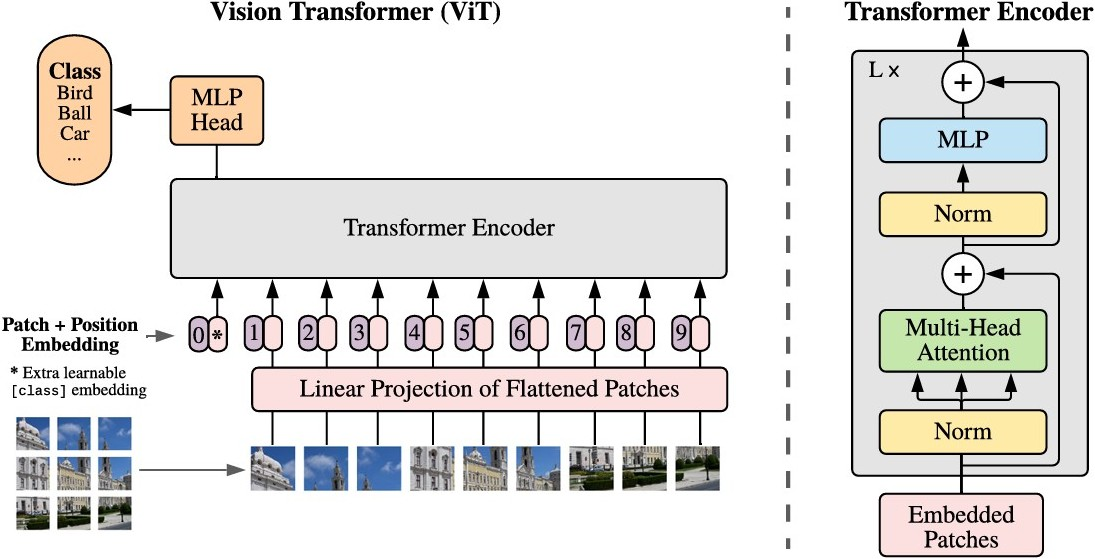
\includegraphics[width=0.9\linewidth]{graphics/ViT-architecture.jpg}
      \caption[Schematischer Aufbau einer Vision Transformer Architektur]{Schematischer Aufbau einer Vision Transformer Architektur\footnotemark }
      \label{fig:vit}
\end{figure}
\footnotetext{Entnommen aus: \cite[S. 3]{dosovitskiy_image_2020}}

Architektonisch wird wie in Abbildung \ref{fig:vit} zu sehen ist bei einem \ac{ViT} das Eingabebild in mehrere Patches zerlegt und diese mittels trainierbarer linearer Projektion in einen Vektor umgewandelt. Dieser Vektor wird um eine Positionsinformation ergänzt und anschließend an den \textit{Transformer Encoder} übergegeben\footnote{Vgl. \cite[3]{dosovitskiy_image_2020}} Durch den Einsatz von \textit{Multi-Head Self-Attention} kann dieser \textit{Encoder} globale Abhängigkeiten zwischen allen Patches modellieren und somit Kontext effektiv bewahren. Durch ein neuronales Netz findet anschließend eine Klassifikation statt.\footnote{Vgl. \cite[3]{dosovitskiy_image_2020}} Der \textit{Transformer Encoder} ist dabei nicht spezifisch auf Bilddaten ausgelegt, sondern könnte auch für andere Sequenzdaten, wie \textit{Text-Embeddings}, verwendet werden.\footnote{Vgl. \cite[3]{dosovitskiy_image_2020}}

Beispielsweise können \acfp{ViT} im Gegensatz zu \acp{CNN} besser globale Bildmerkmale sowie Zusammenhänge verschiedener Elemente bewahren\footnote{Vgl. \cite[S. 206]{berroukham_vision_2023}}, wodurch sie in der Praxis schon erfolgreich Anwendung finden und in Fällen, wie im medizinischen Umfeld zur Erkennung von bestimmten Krankheiten, \acp{CNN} übertreffen.\footnote{Vgl. \cite[S. 208]{berroukham_vision_2023}}

Trotz ihrer Erfolge sind \acp{ViT} mit einer Reihe technischer Herausforderungen verbunden. Hierzu gehören neben höheren Rechenkosten durch eine große Anzahl an Parametern auch die Notwendigkeit von größeren Datensätzen, da diese ansonsten oftmals schlechter als \ac{CNN}-Architekturen abschneiden.\footnote{Vgl. \cite[8]{jamil_comprehensive_2022}} \acp{ViT} sind außerdem stärker davon abhängig, dass Trainingsdaten nicht in schlechter Qualität oder verzerrt vorliegen.\footnote{Vgl. \cite[209]{berroukham_vision_2023}} Die Arbeit von \cite{hutten_vision_2022} zeigt allerdings, dass auch solche Herausforderungen mit geeigneten Transformer-Architekturen adressiert werden können. In ihrer Arbeit wurden verschiedene Modelle zur Anwendbarkeit von \acp{ViT} in der industriellen Inspektion am Beispiel von Güterwagen getestet. Dabei wurden Transformer-Architekturen mit \ac{CNN}-basierten Ansätzen verglichen, indem sie auf dem gleichen, kleinen Datensatz trainiert und evaluiert wurden. Die Transfomer-Modelle erzielten hierbei bessere Ergebnisse als \acp{CNN}, ohne signifikante Unterschiede in der Trainingsgeschwindigkeit aufzuweisen, was die Potenziale von \acp{ViT} auch in datenlimitierten industriellen Umgebungen deutlich unterstreicht.\footnote{Vgl. \cite{hutten_vision_2022}}

%\textcolor{red}{Ich bin mir wegen dem Umfang unsicher, deswegen wurde folgendes Paper nicht aufgenommen, könnte aber intererssant sein: es geht auf eine Hybride Varianten ein und stellt ebenfalls Unterschiede und Vor-/Nachteile von \acp{CNN} bzw. \acp{ViT} heraus. Es enthält auch, wer erste Entwicklungen bei Text- und Bild-Transformern entwickelt hatte: https://doi.org/10.48550/arXiv.2305.09880}

%\textcolor{red}{Zusätzlich noch VLMs nennen?}

%\textcolor{red}{Sollte noch auf Risiken oder Probleme eingangen werden beim Einsatz von KI? z.B. das Problem der Erklärbarkeit, insbesondere in Bezug auf die Nutzung von digitalen Zwillingen im Bereich Predictive Maintenance oder der Fehlerkennung/-klassifizierung}


\section{Fehlererkennung und -klassifikation in der Fertigung}

Die Fehlererkennung und -klassifikation (engl. \textit{\ac{FDD}}) ist keine neue Thematik, sondern wird bereits seit Anfang der 70er Jahre untersucht.\footnote{Vgl. \cite[S. 4]{mercorelli_recent_2024}} Aufgrund der neuen vielversprechenden technischen Entwicklungen, insbesondere im Bereich des \ac{DL}, wird diese Thematik jedoch immer relevanter, insbesondere mit Fokus auf die Implementierung von \ac{KI}-Technologien zur Unterstützung dieses Prozesses.\footnote{Vgl. \cite[S. 1]{seid_ahmed_advances_2025}} Neben der reinen Fehlervermeidung bietet \ac{FDD} durch ein schnelles Erkennen und korrektes Reagieren auf Fehler erhebliche wirtschaftliche Vorteile, wie die Reduktion von Prozesskosten sowie die Steigerung der Produktivität und Qualität in der Fertigung.\footnote{Vgl. \cite[S. 4]{seid_ahmed_advances_2025}}

\subsection{Begriffsdefinition und -abgrenzung}
Die Fehlererkennung (engl. \textit{Fault Detection}) konzentriert sich darauf, festzustellen, ob ein Fehler oder eine Anomalie vorliegt. Anschließend zielt die Fehlerdiagnose (engl. \textit{Fault Diagnostics}) darauf ab, den Fehler in Kategorien bekannter Fehler einzuordnen und somit zu klassifizieren.\footnote{Vgl. \cite[S. 442]{wu_transformer-based_2023}} Dazu gehört außerdem möglichst viel über den Fehler und dessen Ursprung in Erfahrung zu bringen, weshalb man die Fehlerdiagnose üblicherweise als einen mehrstufigen Prozess betrachten kann, welcher die Erkennung, Isolation, Identifizierung sowieso Klassifizierung und Bewertung umfasst.\footnote{Vgl. \cite[S. 12]{mercorelli_recent_2024}; \cite[S. 16]{seid_ahmed_advances_2025}}

\subsection[Kategorien von Fault Detection and Diagnostics (FDD) Methoden]{Kategorien von \ac{FDD} Methoden}
Es wurden viele verschiedene \ac{FDD}-Methoden entwickelt, welche sich in 3 Gruppen einteilen lassen: \textit{Data-driven}, \textit{Model-based} und \textit{Knowledge-based} Methoden. Im Folgenden sollen diese Methoden unterschieden werden\footnote{Vgl. \cite[S. 4]{seid_ahmed_advances_2025}}

\textbf{Datengetriebene Methoden (Data-driven)} 

Datengetriebene Methoden nutzen historische Daten, um durch statistische Techniken oder \textit{Machine Learning}-Algorithmen charakteristische Muster und Abweichungen zu erkennen und dadurch Anomalien und Fehler erkennen und klassifizieren zu können. Diese Verfahren sind deutlich anpassungsfähiger als andere Methoden und können auch komplexe Prozesse überwachen. Sie sind insbesondere dann nützlich, wenn umfangreiche Daten bereits vorliegen. Allerdings zeigt sich hier auch der Nachteil solcher Verfahren, da große, repräsentative Datensätze für das Training solcher Modelle erforderlich sind.\footnote{Vgl. \cite[S. 16 ff.]{mercorelli_recent_2024}}

\textbf{Modellbasierte Methoden (Model-based)}

Diese Verfahren stützen sich auf ein physikalisches oder mathematisches Modell des Systems, aufgrund welchem das erwartete Verhalten berechnet werden kann. Eine Abweichung des tatsächlichen vom erwarteten Verhalten weist auf einen potenziellen Fehler hin und kann zur dessen Identifikation und Klassifikation herangezogen werden. Die größten Herausforderungen sind hierbei der Rechenaufwand sowie das nötige Verständnis über das System. Sind diese Faktoren jedoch gegeben, kann diese Methode sehr präzise sein.\footnote{Vgl. \cite[S. 21 ff.]{mercorelli_recent_2024}}

\textbf{Wissensbasierte Methoden (Knowledge-based)} 

Wissensbasierte Verfahren basieren auf kodiertem Expertenwissen und sind dadurch besonders nützlich, wenn fundiertes Fachwissen vorliegt. Ein wesentlicher Vorteil liegt neben einer hohen Verarbeitungsgeschwindigkeit in der Nachvollziehbarkeit der Entscheidungen des Systems. Bei bislang unbekannten Fehlern sowie unvollständigem oder falschem Expertenwissen stoßen diese Methoden jedoch an ihre Grenzen.\footnote{Vgl. \cite[S. 22 f.]{mercorelli_recent_2024}}

\textbf{Hybride Methoden}

Es existieren außerdem hybride-Verfahren, bei welchen Elemente aus \textit{model-based}, \textit{data-based} und \textit{knowledge-based} Ansätzen kombiniert werden, um jeweilige Stärken zu nutzen und bestehende Schwächen auszugleichen. Dadurch wird das System robuster und flexibler, jedoch kann hier die Integration der verschiedenen Methoden ineinander eine Herausforderung darstellen.\footnote{Vgl. \cite[S. 22 f.]{mercorelli_recent_2024}}

\subsection{Aktuelle Trends}
Aktuelle Trends befinden sich zurzeit vor allem im Bereich der künstlichen Intelligenz. \ac{DL} steht im Bereich der \ac{FDD} immer mehr im Mittelpunkt, um Merkmale aus Rohdaten automatisiert zu extrahieren und die Fehlererkennung und Diagnose voranzutreiben.\footnote{Vgl. \cite[S. 5991]{wen_new_2018}}
Zu den populärsten Anwendungen von \ac{DL} in der \ac{FDD} zählen immer noch \acp{CNN}, um Bilddaten zu analysieren und Degradationsmuster aus Sensordaten zu extrahieren.\footnote{Vgl. \cite{wu_transformer-based_2023}; \cite[S.  5991]{wen_new_2018}} Allerdings zeigt die Forschung aktuell, wie bereits in \ref{sec:ki_modelle_bildverarbeitung} erläutert, ein steigendes Interesse an der Nutzung von \acp{ViT} in der Fertigungsindustrie, welche die Leistung von \acp{CNN} übertreffen können. \acp{ViT} bieten unter anderem durch ihr Aufmerksamkeitsmechanismen ein großes Potenzial beim Umgang mit \ac{FDD}-Daten.\footnote{Vgl. \cite[S. 440]{wu_transformer-based_2023}}Ein wesentlicher Vorteil bei der Nutzung von Transformern besteht zudem in der Möglichkeit zur Neuheitserkennung (engl. \textit{Novel Detection}). Das bedeutet, dass das Modell neue oder unbekannte Fehler identifizieren kann, welche vorher noch nicht beobachtet wurden.

\subsection{Herausforderungen und Forschungsbedarf}
Trotz der erzielten Fortschritte bestehen mehrere zentrale Herausforderungen. Zu diesen gehören wie schon in \ref{sec:synthetische_daten_section} beschrieben, die Notwendigkeit von großen Mengen an annotierten, vielfältigen Daten, was insbesondere im Fertigungsbereich eine aktuelle Problematik darstellt und durch die Generierung von synthetischen Daten in dieser Arbeit adressiert werden soll. Des weiteren stellt die Komplexität und Interpretierbarkeit von Modellen eine aktuelle Herausforderung dar. \ac{DL} Modelle werden oftmals als "Black Boxes" betrachtet, bei welchen dessen Entscheidungslogik nur schwer nachvollzogen werden kann.\footnote{Vgl. \cite[S. 10]{chai_deep_2021}} Eine weitere Herausforderung stellt die Generalisierung solcher Modelle dar. Treten neue Fehler auf, welche beim Training nicht vorhanden waren, werden diese vom Modell inkorrekt klassifiziert.\footnote{Vgl. \cite[S. 440]{wu_transformer-based_2023}}
Aus der Literatur lässt sich damit ein dringender Bedarf an leistungsfähigen \ac{FDD}-Methoden ableiten, insbesondere für eine zuverlässige und echtzeitfähige Fehlerdiagnose in großskaligen Produktionssystemen, sodass weitere Forschung und Entwicklung in diesem Bereich unerlässlich ist.\footnote{Vgl. \cite[S. 4]{seid_ahmed_advances_2025}; \cite[S. 442]{wu_transformer-based_2023}}


\section{Remote Monitoring}

\subsection{Begriffsabgrenzung: Remote Services, Remote Operations, Remote Monitoring}
Der Begriff Remote Services dient als Sammelbegriff für verschiedene Formen der ortsunabhängigen Unterstützung, unter welchen unter anderem die Serviceformen Remote Repair, Remote Maintenance und Remote Operations fallen.\footnote{Vgl. \cite[S. 5]{holtbrugge_remote_2007}}
Unter dem Begriff der Remote Operations versteht man die aktive Fernüberwachung, Ferndiagnose sowie den Fernbetrieb einer Anlage. Remote Monitoring bezeichnet die Fernüberwachung und -diagnose und kann somit als Teil der Remote Operations eingeordnet werden.\footnote{\cite[S. 592 f.]{vogel-heuser_remote_2024}}

\iffalse
\subsection{Differenzierungen von Remote Operations}
Die Namur-Empfehlung NE 161 differenziert Remote Operations in drei Kategorien, welche sich in ihrem Grad der Autonomie unterscheiden:
\begin{itemize}
    \item \textbf{Kategorie 1:} Anlagen werden überwiegend vor Ort gesteuert und überwacht\footnote{\cite[S. 593]{vogel-heuser_remote_2024}}
    \item \textbf{Kategorie 2:} Anlagen können für einen begrenzten Zeitraum aus der Ferne betrieben werden,  beispielsweise in Nacht- oder Wochenendschichten, wodurch nicht jederzeit Personal vor Ort erforderlich ist. Es werden allerdings weiterhin Tätigkeiten vor Ort durchgeführt.\footnote{\cite[S. 593]{vogel-heuser_remote_2024}}
    \item \textbf{Kategorie 3:} Vollständig fernbediente Anlagen, bei denen nur in Ausnahmefällen Personal herangezogen wird. Im Regelfall befindet sich kein Personal in der Anlage.\footnote{\cite[S. 593]{vogel-heuser_remote_2024}}  
\end{itemize}

Die NAMUR-Empfehlung unterscheidet zudem in 3 aufeinander aufbauenden Ebenen: Fernüberwachung, Ferndiagnose und Fernsteuerung:
\begin{itemize}
    \item \textbf{Fernüberwachung:} Kontinuierliche Beobachtung der Anlage, beispielsweise durch KPIs, wobei jedoch keine Diagnose von Fehlern stattfindet.\footnote{\cite[S. 593]{vogel-heuser_remote_2024}}
    \item \textbf{Ferndiagnose:} Baut auf der Fernüberwachung auf und erlaubt neben der Überwachung der Anlage auch eine Analyse und Bewertung der Daten, wobei diese Ebene keine Eingriffe in den tatsächlichen Prozess erlaubt.\footnote{\cite[S. 593]{vogel-heuser_remote_2024}}
    \item \textbf{Fernsteuerung:} Erst auf dieser Ebene sind auch direkte Eingriffe in die Anlage und deren Prozess möglich.\footnote{\cite[S. 593]{vogel-heuser_remote_2024}}
\end{itemize}

Remote Monitoring lässt sich folglich in Kategorie 2 und der Ebene der Fernüberwachung einordnen, da weiterhin Personal vor Ort vorhanden sein muss und keine Eingriffe in den Prozess nicht umfasst sind, sondern ausschließlich die Überwachung und Analyse der erfassten Daten. Remote Operations hingegen kann je nach Ausprägung den Kategorien 2 bis 3 und der Ebene der Fernsteuerung zugeordnet werden.
\fi

\subsection{Remote Monitoring in der Fertigung}
Durch Remote Monitoring wird eine kontinuierliche Überwachung und Analyse der Fertigungsanlage gewährleistet, wodurch Fehlerfälle schneller erkannt und klassifiziert werden können. Dies erleichtert die Fehlerbehebung in den nachfolgenden Schritten, wodurch die Effizienz und Auslastung der Anlage erhöht als auch Kosten eingespart werden können.\footnote{Vgl. \cite[S. 110]{holtbrugge_remote_2007}} Darüber hinaus schafft Remote Monitoring die Grundlage für ferngesteuerten Reparaturen und Instandhaltungen im Rahmen von Remote Operations, wodurch Kosten reduziert werden und das Personal effizienter ausgelastet werden kann.\footnote{Vgl. \cite[S. 5, 110]{holtbrugge_remote_2007}} Remote Services gewinnen zunehmend an Bedeutung, weshalb dieses Themengebiet einen wichtigen Forschungszweig darstellt.\footnote{Vgl. \cite[S. 5]{holtbrugge_remote_2007}}
Auch bei TRUMPF kommt Remote Monitoring zum Einsatz, um Fehler bei Stillständen von Maschinen aus der Ferne identifizieren zu können, um diese anschließend per Fernzugriff zu entstören.

\subsection{Voraussetzungen für Remote Monitoring}
Für die Umsetzung eines effektiven Remote Monitoring Systems ist es nötig, die menschlichen Sinne und menschliche Intelligenz nachzubilden, um Zustände korrekt wahrzunehmen und zu interpretieren.\footnote{Vgl. \cite[S. 596]{vogel-heuser_remote_2024}} Zur Nachbildung der menschlichen Sinne kommen je nach Anwendungsfall verschiedene Sensoren, wie beispielsweise Kameras, Mikrofone, Temperatur- oder Gassensoren, zum Einsatz.\footnote{Vgl. \cite[S. 596 f.]{vogel-heuser_remote_2024}} Um menschliche Intelligenz nachzubilden eignen sich verschiedene Methoden der künstlichen Intelligenz. Die Auswahl des geeigneten Algorithmus richtet sich hierbei ebenfalls nach den spezifischen Anforderungen des Anwendungsfalls.\cite[S. 597]{vogel-heuser_remote_2024}


\section[Evaluationsmethoden für Computer Vision-Modelle]{Evaluationsmethoden für \ac{CV}-Modelle}

\subsection{Grundlagen der Modellevaluation}
\ac{KI} Modelle zu evaluieren ist entscheidend, um ihre Leistung, Zuverlässigkeit und Eignung für den jeweiligen Anwendungsfall beurteilen und verschiedene Modelle vergleichen zu können. Sie ermöglicht zudem den Vergleich unterschiedlicher Modellarchitekturen, wie beispielsweise \acp{CNN} und \acp{ViT}.\footnote{Vgl. \cite[S. 105281]{ali_adversarial_2024}}

Ziel der Modellevaluation ist es, die Leistungsfähigkeit eines Modells quantitativ zu erfassen. Neben der reinen Genauigkeit (engl. \textit{Accuracy}) spielen außerdem weitere Kennzahlen wie Präzision (engl. \textit{Precision}), Sensitivität (engl. \textit{Recall}) und der harmonische Mittelwert dieser beiden, der \textit{\(F1\)-Score}, eine zentrale Rolle, insbesondere bei unausgeglichenen Datensätzen\footnote{Vgl. \cite[S. 65240]{arslanoglu_vision_2025}}. Des weiteren ist die Robustheit von Modellen, also die Fähigkeit, unter variierenden Eingabebedingungen (z.B. Rauschen, Helligkeit, Rotation, Bildqualität, geometrische Unterschiede) konsistente Ergebnisse zu liefern, ebenfalls entscheidend.\footnote{Vgl. \cite[S. 65234]{arslanoglu_vision_2025}} Diese kann durch Tests unter veränderten Bedingungen ermittelt werden.\footnote{Vgl. \cite[S. 323]{zhang_computer_2023}}

\subsection{Zentrale Evaluationsmetriken für die Objekterkennung}

Während die Genauigkeit angibt, welcher Anteil aller Vorhersagen korrekt ist, misst die Präzision (\(P\)) den Anteil der als positiv klassifizierten Vorhersagen, welche auch korrekterweise positiv (engl. \textit{\ac{TP}}) sind.\footnote{Vgl. \cite[S. 65240]{arslanoglu_vision_2025}}
\[
P = \frac{\text{\acs{TP}}}{\text{\acs{TP}} + \text{\acs{FP}}}
\]
Die Sensitivität (\(R\)) hingegen misst den Anteil der korrekt erkannten positiven Instanzen an allen tatsächlich positiven Instanzen, also \acf{TP} + \ac{FN}.\footnote{Vgl. \cite[S. 65240]{arslanoglu_vision_2025}} 
\[
R = \frac{\acs{TP}}{\acs{TP} + \acs{FN}}
\]

Für Objekterkennungsaufgaben werden typischerweise spezifische Metriken eingesetzt, die neben der Klassifikationsleistung auch die Genauigkeit der Lokalisierung berücksichtigen, wie etwa die \ac{AP} oder die daraus abgeleitete \ac{mAP}.\footnote{Vgl. \cite[S. 94272]{khanam_comprehensive_2024}} Grundlage der Bewertung, ob eine Detektion als korrekt gilt, ist die \ac{IoU}, welche den Überlappungsgrad zwischen vorhergesagter und tatsächlicher \textit{Bounding Box} misst.\footnote{Vgl. \cite[S. 94272]{khanam_comprehensive_2024}} Ein gängiger Schwellenwert hierfür ist 0.5, wonach die Detektion als erfolgreich klassifiziert wird, wenn die vorhergesagte und tatsächliche \textit{Bounding Box} um mindestens 50\% übereinstimmen.\footnote{Vgl. \cite[S. 94272]{khanam_comprehensive_2024}}

Die \ac{AP} entspricht der Fläche unter der Precision–Recall-Kurve bei einem festgelegten \ac{IoU}.-Schwellenwert (z.\,B. 0.5. für \ac{AP}50).\footnote{Vgl. \cite[13]{zaripov_creation_2025}}

\[
\acs{AP} = \int_0^1 p(r) \, dr
\]

Die \ac{mAP} ist der Mittelwert der \ac{AP}-Werte über alle Klassen.\footnote{Vgl. \cite[14]{zaripov_creation_2025}} Je nach Evaluationsprotokoll kann zudem über mehrere \ac{IoU}-Schwellenwerte gemittelt werden. In der Praxis wird häufig \ac{mAP}50 verwendet, d.\,h. der Mittelwert der \ac{AP} über alle Klassen bei \ac{IoU}-Schwelle 0.5.\footnote{Vgl. \cite[S. 13 f.]{zaripov_creation_2025}}

In diesem Zusammenhang wird häufig der \ac{mAP}50 verwendet, welcher die \ac{mAP}-Metrik mit Verwendung der \ac{IoU}-Schwelle 0.5 berechnet.\footnote{Vgl. \cite[S. 13]{zaripov_creation_2025}}


\subsection{Vergleich und Auswahl von Metriken}

Die Auswahl geeigneter Evaluationsmetriken hängt maßgeblich von den Datencharakteristika, der Aufgabenstellung und den Prioritäten des Anwendungsfalls ab. In der Objekterkennung hat sich insbesondere die Mean Average Precision (\ac{mAP}) etabliert, da sie sowohl Klassifikations- als auch Lokalisierungsfehler berücksichtigt und damit ein differenziertes Bild der Modellleistung liefert.\footnote{Vgl. \cite[S. 65240]{arslanoglu_vision_2025}; \cite[S. 94272]{khanam_comprehensive_2024}} 

Insbesondere in sicherheitskritischen Bereichen ist es darüber hinaus sinnvoll, die Robustheit eines Modells gegenüber veränderten Eingabebedingungen mit zu berücksichtigen, um ein umfassenderes Bewertungsbild zu erhalten.\footnote{Vgl. \cite[S. 65234]{arslanoglu_vision_2025}; \cite[S. 105282]{ali_adversarial_2024}} Häufig empfiehlt sich daher eine kombinierte Evaluation, bei der mehrere Kennzahlen einbezogen werden, um unterschiedliche Leistungsaspekte des Modells abzudecken.
